\frame{\titlepage}
{
\usebackgroundtemplate{
    \rule{0pt}{\paperheight}
    \hspace*{\paperwidth}
    \makebox[0pt][r]{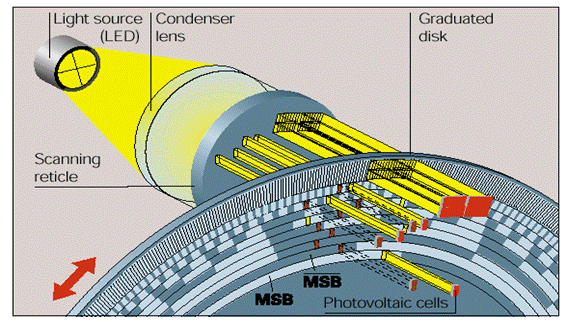
\includegraphics[width=.63\linewidth]{../Figures/encoders.png}}
}
\frame{\frametitle{Содержание}\tableofcontents}
}

\section{Введение}

\begin{frame}{Типичный энкодер}
    \centering
    \begin{figure}[ht]
        \subfloat[]{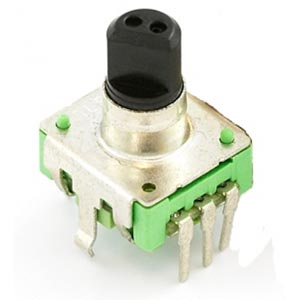
\includegraphics[width=.4\linewidth]{../Figures/encoder.png}}
        \qquad
        \subfloat[]{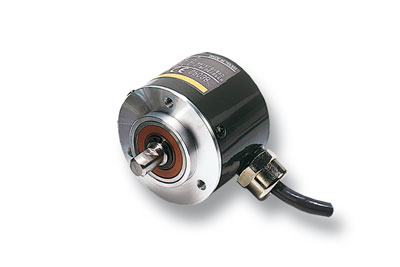
\includegraphics[width=.4\linewidth]{../Figures/indenc.png}}
        \caption{Энкодер (а) бытовой инкрементальный; (б) промышленный позиционный}
    \end{figure}
\end{frame}

\begin{frame}{Сигналы с выходов энкодера}
    \centering
    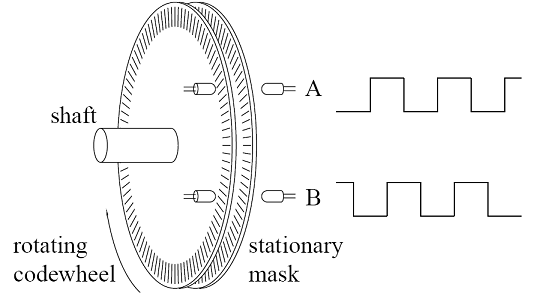
\includegraphics[width=.8\linewidth]{../Figures/meandr.png}
\end{frame}

\section{Устройство энкодера накапливающего типа}

\begin{frame}{Устройство энкодера накапливающего типа}
    \centering
    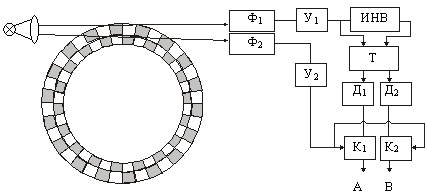
\includegraphics[width=.8\linewidth]{../Figures/disk.png}
    \begin{itemize}
        \pause\item $\textup{Ф}_1$ и $\textup{Ф}_2$ --- фотоприемники;
        \pause\item $\textup{У}_1$ и $\textup{У}_2$ --- усилители;
        \pause\item Т --- триггер;
        \pause\item $\textup{Д}_1$ и $\textup{Д}_2$ --- дифференцирующие элементы (одновибраторы);
        \pause\item $\textup{К}_1$ и $\textup{К}_2$ --- ключи.
    \end{itemize}
\end{frame}

\begin{frame}{Сигналы на элементах}
    \centering
    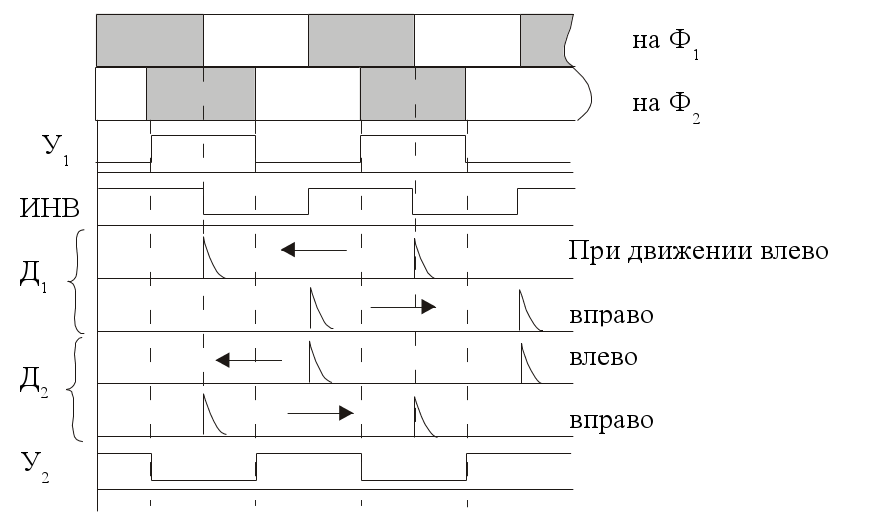
\includegraphics[width=.8\linewidth]{../Figures/complex.png}
\end{frame}

\begin{frame}{Направление вращения}
    \centering
    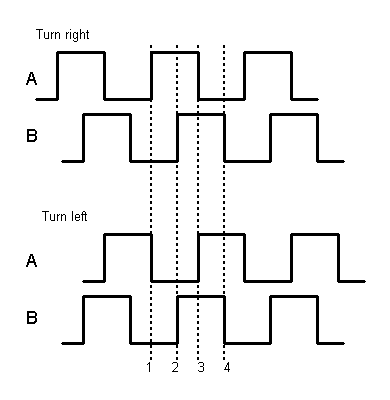
\includegraphics[width=.4\linewidth]{../Figures/reverse.png}
    \qquad
    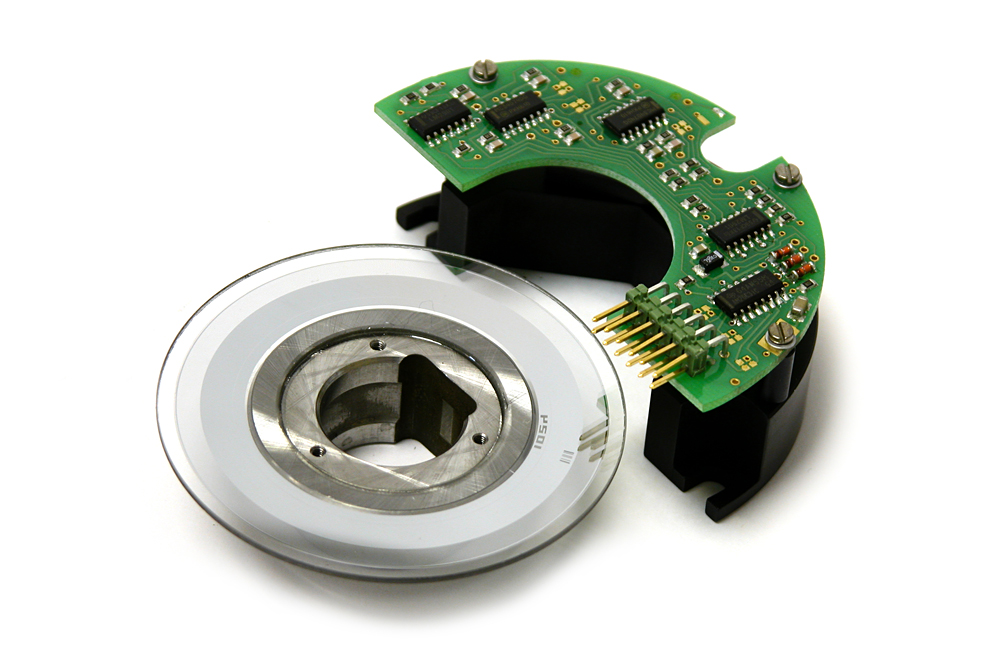
\includegraphics[width=.4\linewidth]{../Figures/splitenc.png}
\end{frame}

\section{Устройство энкодера абсолютного типа}

\begin{frame}{Кодовый диск абсолютного энкодера}
    \centering
    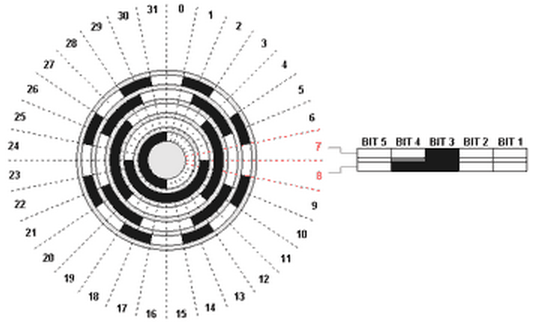
\includegraphics[width=.8\linewidth]{../Figures/code.png}

    $\textrm{Дискретность} = 2^n$, где $n$ --- число дорожек
\end{frame}

\begin{frame}{Двоичный код трехдорожкового энкодера}
    \centering
    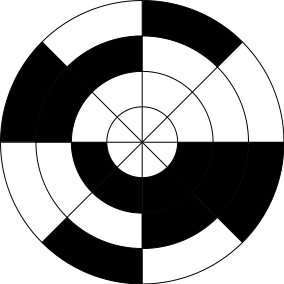
\includegraphics[width=.5\linewidth]{../Figures/3contacts.png}

    $n = 3$, $2^n = 8$ позиций
\end{frame}

\begin{frame}{Стандартная двоичная кодировка}
    \begin{longtable}[c]{|c|c|c|c|c|}
        \hline
        \multirow{2}{*}{\textbf{Сектор}} & \multicolumn{3}{|c|}{\textbf{Номер дорожки}} & \multirow{2}{*}{\textbf{Диапазон}}\\
        \cline{2-4}
        & \textbf{1} & \textbf{2} & \textbf{3} &\\
        \hline
        \endfirsthead
        \hline
        \textbf{Сектор} & \textbf{Дорожка 1} & \textbf{Дорожка 2} & \textbf{Дорожка 3} & \textbf{Диапазон}\\
        \hline
        \endhead
        0 & off & off & off & $0^{\circ}$ -- $45^{\circ}$\\
        \hline
        1 & off & off & \cellcolor{green!20}ON & $45^{\circ}$ -- $90^{\circ}$\\
        \hline
        2 & off & \cellcolor{green!20}ON & off & $90^{\circ}$ -- $135^{\circ}$\\
        \hline
        3 & off & \cellcolor{green!20}ON & \cellcolor{green!20}ON & $135^{\circ}$ -- $180^{\circ}$\\
        \hline
        4 & \cellcolor{green!20}ON & off & off & $180^{\circ}$ -- $225^{\circ}$\\
        \hline
        5 & \cellcolor{green!20}ON & off & \cellcolor{green!20}ON & $225^{\circ}$ -- $270^{\circ}$\\
        \hline
        6 & \cellcolor{green!20}ON & \cellcolor{green!20}ON & off & $270^{\circ}$ -- $315^{\circ}$\\
        \hline
        7 & \cellcolor{green!20}ON & \cellcolor{green!20}ON & \cellcolor{green!20}ON & $315^{\circ}$ -- $360^{\circ}$\\
        \hline
    \end{longtable}
    \begin{exampleblock}{\centeringПереход из третьего сектора в четвертый}
        \centering
        \scriptsize\textbf{\pause{off-on-on}\\\pause{off-on-off}\\\pause{on-on-off}\\\pause{on-off-off}}
    \end{exampleblock}
\end{frame}

\section{Код Грея}

\begin{frame}{Кодировка Грея}
    \begin{longtable}[c]{|c|c|c|c|c|}
        \hline
        \multirow{2}{*}{\textbf{Сектор}} & \multicolumn{3}{|c|}{\textbf{Номер дорожки}} & \multirow{2}{*}{\textbf{Диапазон}}\\
        \cline{2-4}
        & \textbf{1} & \textbf{2} & \textbf{3} &\\
        \hline
        \endfirsthead
        \hline
        \textbf{Сектор} & \textbf{Дорожка 1} & \textbf{Дорожка 2} & \textbf{Дорожка 3} & \textbf{Диапазон}\\
        \hline
        \endhead
        0 & off & off & off & $0^{\circ}$ -- $45^{\circ}$\\
        \hline
        1 & off & off & \cellcolor{green!20}ON & $45^{\circ}$ -- $90^{\circ}$\\
        \hline
        2 & off & \cellcolor{green!20}ON & \cellcolor{green!20}ON & $90^{\circ}$ -- $135^{\circ}$\\
        \hline
        3 & off & \cellcolor{green!20}ON & off & $135^{\circ}$ -- $180^{\circ}$\\
        \hline
        4 & \cellcolor{green!20}ON & \cellcolor{green!20}ON & off & $180^{\circ}$ -- $225^{\circ}$\\
        \hline
        5 & \cellcolor{green!20}ON & \cellcolor{green!20}ON & \cellcolor{green!20}ON & $225^{\circ}$ -- $270^{\circ}$\\
        \hline
        6 & \cellcolor{green!20}ON & off & \cellcolor{green!20}ON & $270^{\circ}$ -- $315^{\circ}$\\
        \hline
        7 & \cellcolor{green!20}ON & off & off & $315^{\circ}$ -- $360^{\circ}$\\
        \hline
    \end{longtable}
\end{frame}

\begin{frame}{Перевод из двоичного кода в код Грея}
    \centering
    $\begin{matrix}
        \pause{G_i = B_i \oplus B_{i+1}} & \pause{B_i = B_{i+1} \oplus G} & \pause{B_k = \bigoplus\limits_{i=k}^N G_i}
    \end{matrix}$

    \pause
    \begin{longtable}[c]{|c|c|c|}
        \hline
        \textbf{Десятичное число} & \textbf{Двоичный код} & \textbf{Код Грея}\\
        \hline
        \endfirsthead
        \hline
        \textbf{Десятичное число} & \textbf{Двоичный код} & \textbf{Код Грея}\\
        \hline
        \endhead
        1 & 0001 & 0001\\
        \hline
        2 & 0010 & 0011\\
        \hline
        3 & 0011 & 0010\\
        \hline
        4 & 0100 & 0110\\
        \hline
        5 & 0101 & 0111\\
        \hline
    \end{longtable}
    $\begin{matrix}
        0101 & \underline{1100101}\\
        \underline{0010} & 1000110\\
        0111
    \end{matrix}$

    \pause
    \large{Маски двоичного кода и кода Грея}

    \visible<6>{
    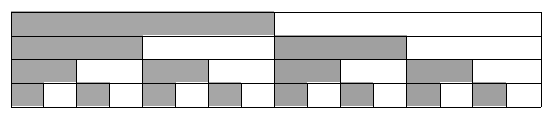
\includegraphics[width=.4\linewidth]{../Figures/binarymask.png}
    \qquad
    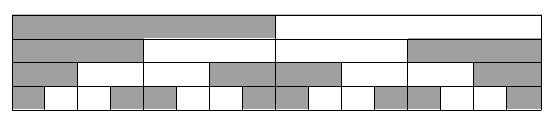
\includegraphics[width=.4\linewidth]{../Figures/cyclemask.png}
    }
\end{frame}

\begin{frame}{Схема преобразователя}
    \centering
    \begin{columns}
        \column{.6\textwidth}
        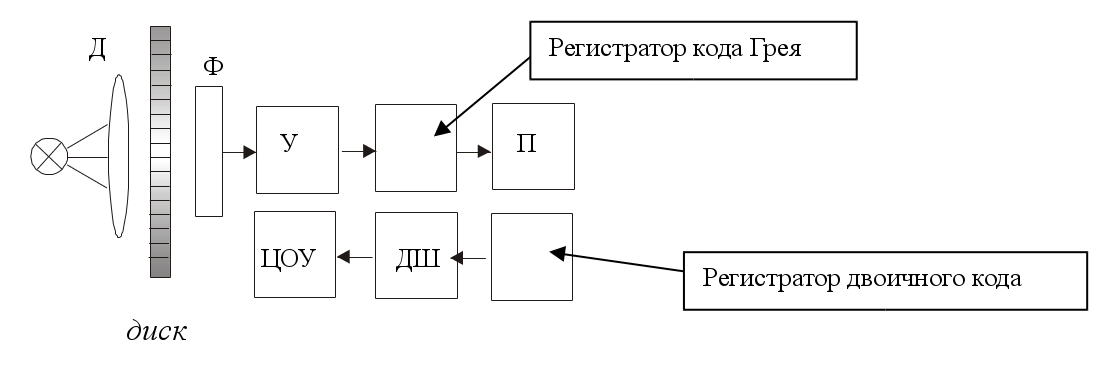
\includegraphics[width=1\linewidth]{../Figures/commonchanger.png}
        {\footnotesize
            \begin{itemize}
                \item Д --- диафрагма;
                \item Ф --- фотоприёмник;
                \item П --- преобразователь;
                \item ДШ --- дешифратор;
                \item ЦОУ --- цифровое отсчетное устройство.
            \end{itemize}
        }
        \column{.4\textwidth}
        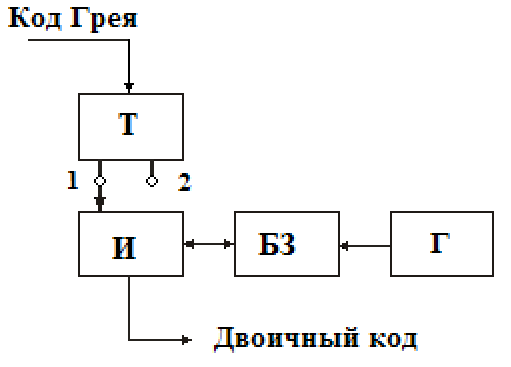
\includegraphics[width=.6\linewidth]{../Figures/changer.png}
        {\scriptsize
            \begin{itemize}
                \item Т --- триггер;
                \item 1 --- сигнал с выхода триггера;
                \item 2 --- для получения инверсного сигнала;
                \item И --- логический элемент ``И'';
                \item Г --- импульсный генератор;
                \item БЗ --- блок задержки.
            \end{itemize}
        }
    \end{columns}
\end{frame}

\begin{frame}{Схема на логических элементах}
    \centering
    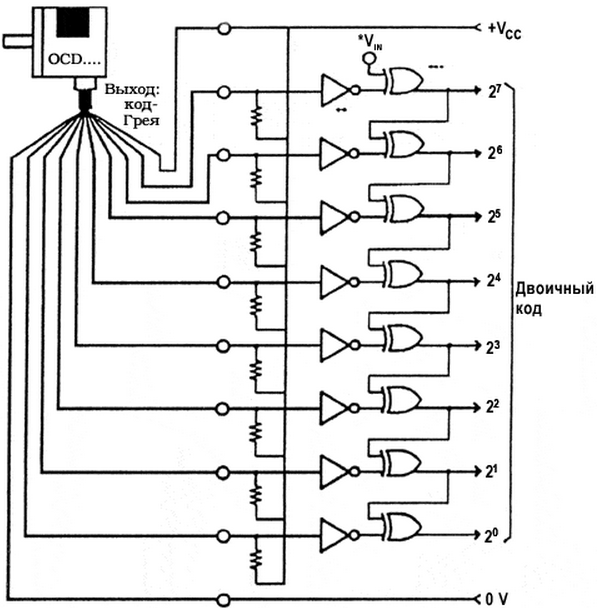
\includegraphics[height=.8\textheight]{../Figures/complexchanger.png}
\end{frame}

\section{Применение энкодеров}

\begin{frame}{Подключение энкодера}
    \centering
    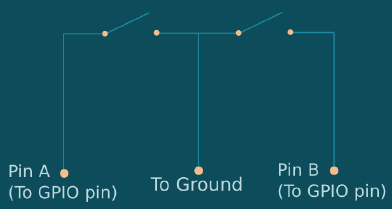
\includegraphics[width=.5\linewidth]{../Figures/pins.png}
    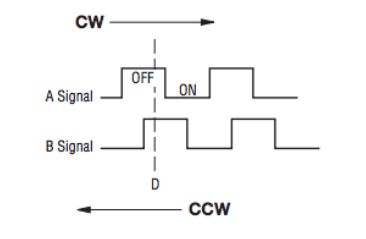
\includegraphics[width=.5\linewidth]{../Figures/signals.png}

    \textbf{GPIO} - General-Purpose Input/Output
\end{frame}

\begin{frame}[fragile]{Определение направления вращения}
    \begin{longtable}[c]{|c|c|c|c|c|}
        \hline
        \textbf{Последовательность} & \textbf{A} & \textbf{B} & \textbf{$A\land B$ (C)} & \textbf{Значение}\\
        \hline
        \endfirsthead
        \hline
        \textbf{Последовательность} & \textbf{A} & \textbf{B} & \textbf{$A^B$ (C)} & \textbf{Значение}\\
        \hline
        \endhead
            0 & 0 & 0 & 0 & 0\\
            \hline
            1 & 1 & 0 & 1 & 5\\
            \hline
            2 & 1 & 1 & 0 & 6\\
            \hline
            3 & 0 & 1 & 1 & 3\\
            \hline
    \end{longtable}

    \centering
    \pause\verb|delta = (new\_state - last\_state) \% 4\end|

\end{frame}

\section{Заключение}

{
\usebackgroundtemplate{
\includegraphics[width=\paperwidth]{../Figures/thanks.png}}
\begin{frame}
    \centering
    \vfill
    \large{Презентация была создана средствами {\LaTeX} и Beamer}
\end{frame}
}
